% Options for packages loaded elsewhere
\PassOptionsToPackage{unicode}{hyperref}
\PassOptionsToPackage{hyphens}{url}
\PassOptionsToPackage{dvipsnames,svgnames,x11names}{xcolor}
%
\documentclass[
  letterpaper,
  DIV=11,
  numbers=noendperiod]{scrartcl}

\usepackage{amsmath,amssymb}
\usepackage{iftex}
\ifPDFTeX
  \usepackage[T1]{fontenc}
  \usepackage[utf8]{inputenc}
  \usepackage{textcomp} % provide euro and other symbols
\else % if luatex or xetex
  \usepackage{unicode-math}
  \defaultfontfeatures{Scale=MatchLowercase}
  \defaultfontfeatures[\rmfamily]{Ligatures=TeX,Scale=1}
\fi
\usepackage{lmodern}
\ifPDFTeX\else  
    % xetex/luatex font selection
\fi
% Use upquote if available, for straight quotes in verbatim environments
\IfFileExists{upquote.sty}{\usepackage{upquote}}{}
\IfFileExists{microtype.sty}{% use microtype if available
  \usepackage[]{microtype}
  \UseMicrotypeSet[protrusion]{basicmath} % disable protrusion for tt fonts
}{}
\makeatletter
\@ifundefined{KOMAClassName}{% if non-KOMA class
  \IfFileExists{parskip.sty}{%
    \usepackage{parskip}
  }{% else
    \setlength{\parindent}{0pt}
    \setlength{\parskip}{6pt plus 2pt minus 1pt}}
}{% if KOMA class
  \KOMAoptions{parskip=half}}
\makeatother
\usepackage{xcolor}
\setlength{\emergencystretch}{3em} % prevent overfull lines
\setcounter{secnumdepth}{-\maxdimen} % remove section numbering
% Make \paragraph and \subparagraph free-standing
\makeatletter
\ifx\paragraph\undefined\else
  \let\oldparagraph\paragraph
  \renewcommand{\paragraph}{
    \@ifstar
      \xxxParagraphStar
      \xxxParagraphNoStar
  }
  \newcommand{\xxxParagraphStar}[1]{\oldparagraph*{#1}\mbox{}}
  \newcommand{\xxxParagraphNoStar}[1]{\oldparagraph{#1}\mbox{}}
\fi
\ifx\subparagraph\undefined\else
  \let\oldsubparagraph\subparagraph
  \renewcommand{\subparagraph}{
    \@ifstar
      \xxxSubParagraphStar
      \xxxSubParagraphNoStar
  }
  \newcommand{\xxxSubParagraphStar}[1]{\oldsubparagraph*{#1}\mbox{}}
  \newcommand{\xxxSubParagraphNoStar}[1]{\oldsubparagraph{#1}\mbox{}}
\fi
\makeatother

\usepackage{color}
\usepackage{fancyvrb}
\newcommand{\VerbBar}{|}
\newcommand{\VERB}{\Verb[commandchars=\\\{\}]}
\DefineVerbatimEnvironment{Highlighting}{Verbatim}{commandchars=\\\{\}}
% Add ',fontsize=\small' for more characters per line
\usepackage{framed}
\definecolor{shadecolor}{RGB}{241,243,245}
\newenvironment{Shaded}{\begin{snugshade}}{\end{snugshade}}
\newcommand{\AlertTok}[1]{\textcolor[rgb]{0.68,0.00,0.00}{#1}}
\newcommand{\AnnotationTok}[1]{\textcolor[rgb]{0.37,0.37,0.37}{#1}}
\newcommand{\AttributeTok}[1]{\textcolor[rgb]{0.40,0.45,0.13}{#1}}
\newcommand{\BaseNTok}[1]{\textcolor[rgb]{0.68,0.00,0.00}{#1}}
\newcommand{\BuiltInTok}[1]{\textcolor[rgb]{0.00,0.23,0.31}{#1}}
\newcommand{\CharTok}[1]{\textcolor[rgb]{0.13,0.47,0.30}{#1}}
\newcommand{\CommentTok}[1]{\textcolor[rgb]{0.37,0.37,0.37}{#1}}
\newcommand{\CommentVarTok}[1]{\textcolor[rgb]{0.37,0.37,0.37}{\textit{#1}}}
\newcommand{\ConstantTok}[1]{\textcolor[rgb]{0.56,0.35,0.01}{#1}}
\newcommand{\ControlFlowTok}[1]{\textcolor[rgb]{0.00,0.23,0.31}{\textbf{#1}}}
\newcommand{\DataTypeTok}[1]{\textcolor[rgb]{0.68,0.00,0.00}{#1}}
\newcommand{\DecValTok}[1]{\textcolor[rgb]{0.68,0.00,0.00}{#1}}
\newcommand{\DocumentationTok}[1]{\textcolor[rgb]{0.37,0.37,0.37}{\textit{#1}}}
\newcommand{\ErrorTok}[1]{\textcolor[rgb]{0.68,0.00,0.00}{#1}}
\newcommand{\ExtensionTok}[1]{\textcolor[rgb]{0.00,0.23,0.31}{#1}}
\newcommand{\FloatTok}[1]{\textcolor[rgb]{0.68,0.00,0.00}{#1}}
\newcommand{\FunctionTok}[1]{\textcolor[rgb]{0.28,0.35,0.67}{#1}}
\newcommand{\ImportTok}[1]{\textcolor[rgb]{0.00,0.46,0.62}{#1}}
\newcommand{\InformationTok}[1]{\textcolor[rgb]{0.37,0.37,0.37}{#1}}
\newcommand{\KeywordTok}[1]{\textcolor[rgb]{0.00,0.23,0.31}{\textbf{#1}}}
\newcommand{\NormalTok}[1]{\textcolor[rgb]{0.00,0.23,0.31}{#1}}
\newcommand{\OperatorTok}[1]{\textcolor[rgb]{0.37,0.37,0.37}{#1}}
\newcommand{\OtherTok}[1]{\textcolor[rgb]{0.00,0.23,0.31}{#1}}
\newcommand{\PreprocessorTok}[1]{\textcolor[rgb]{0.68,0.00,0.00}{#1}}
\newcommand{\RegionMarkerTok}[1]{\textcolor[rgb]{0.00,0.23,0.31}{#1}}
\newcommand{\SpecialCharTok}[1]{\textcolor[rgb]{0.37,0.37,0.37}{#1}}
\newcommand{\SpecialStringTok}[1]{\textcolor[rgb]{0.13,0.47,0.30}{#1}}
\newcommand{\StringTok}[1]{\textcolor[rgb]{0.13,0.47,0.30}{#1}}
\newcommand{\VariableTok}[1]{\textcolor[rgb]{0.07,0.07,0.07}{#1}}
\newcommand{\VerbatimStringTok}[1]{\textcolor[rgb]{0.13,0.47,0.30}{#1}}
\newcommand{\WarningTok}[1]{\textcolor[rgb]{0.37,0.37,0.37}{\textit{#1}}}

\providecommand{\tightlist}{%
  \setlength{\itemsep}{0pt}\setlength{\parskip}{0pt}}\usepackage{longtable,booktabs,array}
\usepackage{calc} % for calculating minipage widths
% Correct order of tables after \paragraph or \subparagraph
\usepackage{etoolbox}
\makeatletter
\patchcmd\longtable{\par}{\if@noskipsec\mbox{}\fi\par}{}{}
\makeatother
% Allow footnotes in longtable head/foot
\IfFileExists{footnotehyper.sty}{\usepackage{footnotehyper}}{\usepackage{footnote}}
\makesavenoteenv{longtable}
\usepackage{graphicx}
\makeatletter
\def\maxwidth{\ifdim\Gin@nat@width>\linewidth\linewidth\else\Gin@nat@width\fi}
\def\maxheight{\ifdim\Gin@nat@height>\textheight\textheight\else\Gin@nat@height\fi}
\makeatother
% Scale images if necessary, so that they will not overflow the page
% margins by default, and it is still possible to overwrite the defaults
% using explicit options in \includegraphics[width, height, ...]{}
\setkeys{Gin}{width=\maxwidth,height=\maxheight,keepaspectratio}
% Set default figure placement to htbp
\makeatletter
\def\fps@figure{htbp}
\makeatother

\KOMAoption{captions}{tableheading}
\makeatletter
\@ifpackageloaded{caption}{}{\usepackage{caption}}
\AtBeginDocument{%
\ifdefined\contentsname
  \renewcommand*\contentsname{Índice}
\else
  \newcommand\contentsname{Índice}
\fi
\ifdefined\listfigurename
  \renewcommand*\listfigurename{Lista de Figuras}
\else
  \newcommand\listfigurename{Lista de Figuras}
\fi
\ifdefined\listtablename
  \renewcommand*\listtablename{Lista de Tabelas}
\else
  \newcommand\listtablename{Lista de Tabelas}
\fi
\ifdefined\figurename
  \renewcommand*\figurename{Figura}
\else
  \newcommand\figurename{Figura}
\fi
\ifdefined\tablename
  \renewcommand*\tablename{Tabela}
\else
  \newcommand\tablename{Tabela}
\fi
}
\@ifpackageloaded{float}{}{\usepackage{float}}
\floatstyle{ruled}
\@ifundefined{c@chapter}{\newfloat{codelisting}{h}{lop}}{\newfloat{codelisting}{h}{lop}[chapter]}
\floatname{codelisting}{Listagem}
\newcommand*\listoflistings{\listof{codelisting}{Lista de Listagens}}
\makeatother
\makeatletter
\makeatother
\makeatletter
\@ifpackageloaded{caption}{}{\usepackage{caption}}
\@ifpackageloaded{subcaption}{}{\usepackage{subcaption}}
\makeatother

\ifLuaTeX
\usepackage[bidi=basic]{babel}
\else
\usepackage[bidi=default]{babel}
\fi
\babelprovide[main,import]{brazilian}
% get rid of language-specific shorthands (see #6817):
\let\LanguageShortHands\languageshorthands
\def\languageshorthands#1{}
\ifLuaTeX
  \usepackage{selnolig}  % disable illegal ligatures
\fi
\usepackage{bookmark}

\IfFileExists{xurl.sty}{\usepackage{xurl}}{} % add URL line breaks if available
\urlstyle{same} % disable monospaced font for URLs
\hypersetup{
  pdftitle={Atividade 3},
  pdfauthor={Mikael Marin Coletto},
  pdflang={pt-BR},
  colorlinks=true,
  linkcolor={blue},
  filecolor={Maroon},
  citecolor={Blue},
  urlcolor={Blue},
  pdfcreator={LaTeX via pandoc}}


\title{Atividade 3}
\author{Mikael Marin Coletto}
\date{2024-12-12}

\begin{document}
\maketitle

\renewcommand*\contentsname{Índice}
{
\hypersetup{linkcolor=}
\setcounter{tocdepth}{3}
\tableofcontents
}

\section{Questão 1}\label{questuxe3o-1}

Dois tipos de solução química, A e B, foram ensaiadas para a
determinação do Ph. As análises de 10 amostras de cada solução estão
apresentadas na tabela que segue. Verifique se há diferença entre elas
(\(\alpha\)=5\%).

A 7,49 7,35 7,54 7,48 7,48 7,37 7,51 7,50 7,52 7,56

B 7,28 7,35 7,52 7,50 7,38 7,48 7,31 7,22 7,41 7,45

\textbf{R:} O teste de Mann-Whitney analisa duas amostras e verifica se
os tratamentos diferente entre si.

H0: As duas soluções não diferem. (Grupo A = Grupo B) H1: As duas
soluções diferem. (Grupo A \(\neq\) Grupo B)

\begin{Shaded}
\begin{Highlighting}[]
\DocumentationTok{\#\# Dados}
\CommentTok{\# Dados do grupo A e B}
\NormalTok{A }\OtherTok{\textless{}{-}} \FunctionTok{c}\NormalTok{(}\FloatTok{7.49}\NormalTok{, }\FloatTok{7.35}\NormalTok{, }\FloatTok{7.54}\NormalTok{, }\FloatTok{7.48}\NormalTok{, }\FloatTok{7.48}\NormalTok{, }\FloatTok{7.37}\NormalTok{, }\FloatTok{7.51}\NormalTok{, }\FloatTok{7.50}\NormalTok{, }\FloatTok{7.52}\NormalTok{, }\FloatTok{7.56}\NormalTok{)}
\NormalTok{B }\OtherTok{\textless{}{-}} \FunctionTok{c}\NormalTok{(}\FloatTok{7.28}\NormalTok{, }\FloatTok{7.35}\NormalTok{, }\FloatTok{7.52}\NormalTok{, }\FloatTok{7.50}\NormalTok{, }\FloatTok{7.38}\NormalTok{, }\FloatTok{7.48}\NormalTok{, }\FloatTok{7.31}\NormalTok{, }\FloatTok{7.22}\NormalTok{, }\FloatTok{7.41}\NormalTok{, }\FloatTok{7.45}\NormalTok{)}

\NormalTok{teste }\OtherTok{\textless{}{-}} \FunctionTok{wilcox.test}\NormalTok{(A, B, }\AttributeTok{alternative =} \StringTok{"two.sided"}\NormalTok{, }\AttributeTok{paired =} \ConstantTok{FALSE}\NormalTok{)}
\end{Highlighting}
\end{Shaded}

\begin{verbatim}
Warning in wilcox.test.default(A, B, alternative = "two.sided", paired =
FALSE): cannot compute exact p-value with ties
\end{verbatim}

\begin{Shaded}
\begin{Highlighting}[]
\NormalTok{teste}
\end{Highlighting}
\end{Shaded}

\begin{verbatim}

    Wilcoxon rank sum test with continuity correction

data:  A and B
W = 77.5, p-value = 0.04072
alternative hypothesis: true location shift is not equal to 0
\end{verbatim}

Usando o nível de significância de 5\%, Tivemos então um p-valor de
0.040717 e como ele é menor que 0.05 (nível de significância de 5\%),
rejeitamos a hipótese nula. Ou seja, há evidências para rejeitar a
hipótese de que os tratamentos não diferem. Portanto, podemos dizer que
as duas soluções químicas não são equivalentes.

\section{Questão 2}\label{questuxe3o-2}

Numa classe de 24 alunos, comparou-se o rendimento de estudantes
provenientes de escolas particulares e escolas públicas. Existe
diferença entre os alunos, à um nível de significância de 10\%?

\begin{figure}[H]

{\centering 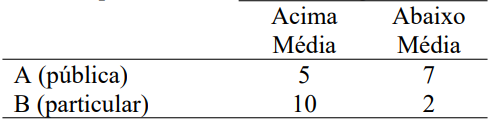
\includegraphics{imgs/q2-tabela.png}

}

\caption{Tabela 2}

\end{figure}%

\textbf{R:} Para estes dados, usaremos o teste exato de Fisher para
verificar se há diferença entre os rendimentos dos alunos de escolas
públicas e particulares.

H0: Os rendimentos das escolas não diferem. (escola pública = escola
particular)

H1: Os rendimentos das escolas diferem. (antes do programa \(\neq\)
depois do programa)

\begin{Shaded}
\begin{Highlighting}[]
\DocumentationTok{\#\# Dados}

\NormalTok{dados  }\OtherTok{\textless{}{-}}
  \FunctionTok{matrix}\NormalTok{(}\FunctionTok{c}\NormalTok{(}\DecValTok{5}\NormalTok{, }\DecValTok{7}\NormalTok{, }\DecValTok{10}\NormalTok{, }\DecValTok{2}\NormalTok{),}
         \AttributeTok{nrow =} \DecValTok{2}\NormalTok{,}
         \AttributeTok{dimnames =} \FunctionTok{list}\NormalTok{(}\AttributeTok{Notas =} \FunctionTok{c}\NormalTok{(}\StringTok{"Acima da média"}\NormalTok{, }\StringTok{"Abaixo da média"}\NormalTok{),}
                         \AttributeTok{Escolas =} \FunctionTok{c}\NormalTok{(}\StringTok{"Pública"}\NormalTok{, }\StringTok{"Particular"}\NormalTok{)))}

\DocumentationTok{\#\# Teste exato de fisher}
\NormalTok{teste }\OtherTok{\textless{}{-}} \FunctionTok{fisher.test}\NormalTok{(dados)}
\NormalTok{teste}
\end{Highlighting}
\end{Shaded}

\begin{verbatim}

    Fisher's Exact Test for Count Data

data:  dados
p-value = 0.08938
alternative hypothesis: true odds ratio is not equal to 1
95 percent confidence interval:
 0.01167257 1.23485892
sample estimates:
odds ratio 
 0.1563843 
\end{verbatim}

O teste nos resultou um p-valor de 0.0893795 e como ele é menor que 0.10
(nível de significância), rejeitamos a hipótese nula. Ou seja, há
evidências para rejeitar a hipótese de que os rendimentos não diferem.
Portanto, podemos dizer que com base no teste exato de Fisher, usando um
p-valor de 10\%, as escolas obtiveram rendimentos diferentes.

\section{Questão 3}\label{questuxe3o-3}

O tempo de uso de um aparelho de um laboratório, em meses, antes de
ocorrer o primeiro defeito, foi anotado para 8 aparelhos da marca A e 10
aparelhos da marca B. Os resultados foram:

\begin{figure}[H]

{\centering 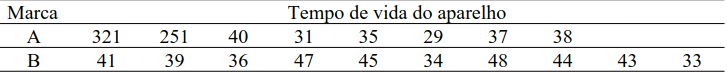
\includegraphics{imgs/q3-tabela.png}

}

\caption{Tabela 3}

\end{figure}%

\textbf{R:} Para estes dados, usaremos o teste de Mann-Whitney para
verificar se há diferença entre os tempos de uso dos aparelhos das
marcas A e B.

H0: Os tratamentos não diferem. (antes do medicamento = depois do
medicamento)

H1: Os tratamentos diferem. (antes do medicamento \(\neq\) depois do
medicamento)

\begin{Shaded}
\begin{Highlighting}[]
\DocumentationTok{\#\# Dados}
\NormalTok{A }\OtherTok{\textless{}{-}} \FunctionTok{c}\NormalTok{(}\DecValTok{321}\NormalTok{, }\DecValTok{251}\NormalTok{, }\DecValTok{40}\NormalTok{, }\DecValTok{31}\NormalTok{, }\DecValTok{35}\NormalTok{, }\DecValTok{29}\NormalTok{, }\DecValTok{37}\NormalTok{, }\DecValTok{38}\NormalTok{)}
\NormalTok{B }\OtherTok{\textless{}{-}} \FunctionTok{c}\NormalTok{(}\DecValTok{41}\NormalTok{, }\DecValTok{39}\NormalTok{, }\DecValTok{36}\NormalTok{, }\DecValTok{47}\NormalTok{, }\DecValTok{45}\NormalTok{, }\DecValTok{34}\NormalTok{, }\DecValTok{48}\NormalTok{, }\DecValTok{44}\NormalTok{, }\DecValTok{43}\NormalTok{, }\DecValTok{33}\NormalTok{)}


\DocumentationTok{\#\# Teste de Mann Whitney}
\NormalTok{teste }\OtherTok{\textless{}{-}} \FunctionTok{wilcox.test}\NormalTok{(A, B, }\AttributeTok{paired =} \ConstantTok{FALSE}\NormalTok{, }\AttributeTok{alternative =} \StringTok{"two.sided"}\NormalTok{)}
\NormalTok{teste}
\end{Highlighting}
\end{Shaded}

\begin{verbatim}

    Wilcoxon rank sum exact test

data:  A and B
W = 32, p-value = 0.5148
alternative hypothesis: true location shift is not equal to 0
\end{verbatim}

Então um p-valor de 0.5147859 e como ele é menor que 0.05, rejeitamos a
hipótese nula (à um nível de significância de 5\%). Ou seja, há
evidências para rejeitar a hipótese de que os tratamentos não diferem.
Portanto, podemos dizer que o medicamento teve um efeito significativo
na pressão arterial diastólica dos pacientes.

\section{Questão 4}\label{questuxe3o-4}

O diretor de uma escola elementar classifica os pais em três categorias
de renda, segundo a área residencial, e em três níveis de participação
nos programas da escola. De acordo com a tabela abaixo, testar a
hipótese de que não existe relação entre renda e participação nos
programas da escola, utilizando um nível de significância de 5\%.
Interprete o significado do resultado do teste.

\begin{figure}[H]

{\centering 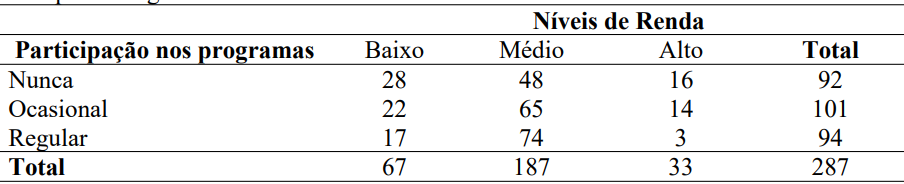
\includegraphics{imgs/q4-tabela.png}

}

\caption{Tabela 4}

\end{figure}%

\textbf{R:} Para estes dados, aplicaremos o teste de qui-quadrado para
verificar se existe diferença entre os níveis de renda e a participação
nos programas da escola.

H0: Os níveis de renda não interfere na participação do programa (baixo
= médio = alto).

H1: Os níveis de renda interfere na participação do programa (pelo menos
uma renda difere das demais).

\begin{Shaded}
\begin{Highlighting}[]
\DocumentationTok{\#\# Dados}
\NormalTok{table\_data }\OtherTok{\textless{}{-}} \FunctionTok{matrix}\NormalTok{(}
  \FunctionTok{c}\NormalTok{(}
    \DecValTok{28}\NormalTok{, }\DecValTok{48}\NormalTok{, }\DecValTok{16}\NormalTok{,  }\CommentTok{\# Frequências para "Nunca"}
    \DecValTok{22}\NormalTok{, }\DecValTok{65}\NormalTok{, }\DecValTok{14}\NormalTok{,  }\CommentTok{\# Frequências para "Ocasional"}
    \DecValTok{17}\NormalTok{, }\DecValTok{74}\NormalTok{, }\DecValTok{3}    \CommentTok{\# Frequências para "Regular"}
\NormalTok{  ),}
  \AttributeTok{nrow =} \DecValTok{3}\NormalTok{, }\AttributeTok{byrow =} \ConstantTok{TRUE}\NormalTok{,}
  \AttributeTok{dimnames =} \FunctionTok{list}\NormalTok{(}
    \AttributeTok{Participacao =} \FunctionTok{c}\NormalTok{(}\StringTok{"Nunca"}\NormalTok{, }\StringTok{"Ocasional"}\NormalTok{, }\StringTok{"Regular"}\NormalTok{),}
    \AttributeTok{Nivel\_de\_Renda =} \FunctionTok{c}\NormalTok{(}\StringTok{"Baixo"}\NormalTok{, }\StringTok{"Medio"}\NormalTok{, }\StringTok{"Alto"}\NormalTok{)}
\NormalTok{  )}
\NormalTok{)}

\CommentTok{\# Convert the matrix to a table object}
\NormalTok{table\_data }\OtherTok{\textless{}{-}} \FunctionTok{as.table}\NormalTok{(table\_data)}

\NormalTok{teste }\OtherTok{\textless{}{-}} \FunctionTok{chisq.test}\NormalTok{(table\_data, }\AttributeTok{correct =}\NormalTok{ F)}
\NormalTok{teste}
\end{Highlighting}
\end{Shaded}

\begin{verbatim}

    Pearson's Chi-squared test

data:  table_data
X-squared = 17.156, df = 4, p-value = 0.001803
\end{verbatim}

Usando o nível de significância de 5\%, Tivemos então um p-valor de
0.0018026 e como ele é menor que 0.05, rejeitamos a hipótese nula. Ou
seja, podemos dizer que existe diferença para pelo menos uma das rendas
em relação às demais no quesito participação nos programas.

\section{Questão 5}\label{questuxe3o-5}

A tabela abaixo faz parte de um estudo que investiga a efetividade dos
capacetes de segurança de bicicleta na prevenção de lesões na cabeça. Os
dados consistem de uma amostra aleatória de 793 indivíduos envolvidos em
acidentes ciclísticos durante um período especificado de um ano.

\begin{figure}[H]

{\centering 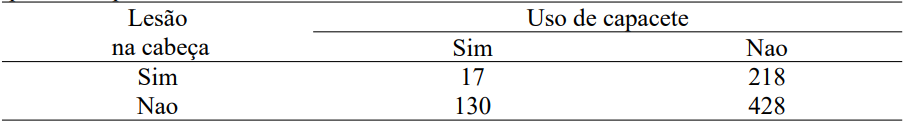
\includegraphics{imgs/q5-tabela.png}

}

\caption{Tabela 5}

\end{figure}%

\textbf{R:} Para estes dados usaremos o teste exato de Fisher para
verificar se há diferença entre o uso de capacete e a efetividade da
segurança das lesões na cabeça.

H0: O uso de capacete não faz diferença significativa na efetividade da
segurança das lesões na cabeça (Com capacete = Sem capacete).

H1: O uso de capacete faz diferença significativa na efetividade da
segurança das lesões na cabeça (Com capacete \(\neq\) Sem capacete).

\begin{Shaded}
\begin{Highlighting}[]
\DocumentationTok{\#\# Dados}
\NormalTok{table\_data }\OtherTok{\textless{}{-}} \FunctionTok{matrix}\NormalTok{(}
  \FunctionTok{c}\NormalTok{(}
    \DecValTok{17}\NormalTok{, }\DecValTok{218}\NormalTok{,  }\CommentTok{\# Frequências para "Sim" (Lesão na cabeça)}
    \DecValTok{130}\NormalTok{, }\DecValTok{428}  \CommentTok{\# Frequências para "Não" (Lesão na cabeça)}
\NormalTok{  ),}
  \AttributeTok{nrow =} \DecValTok{2}\NormalTok{, }\AttributeTok{byrow =} \ConstantTok{TRUE}\NormalTok{,}
  \AttributeTok{dimnames =} \FunctionTok{list}\NormalTok{(}
    \AttributeTok{Lesao\_na\_Cabeca =} \FunctionTok{c}\NormalTok{(}\StringTok{"Sim"}\NormalTok{, }\StringTok{"Nao"}\NormalTok{),}
    \AttributeTok{Uso\_de\_Capacete =} \FunctionTok{c}\NormalTok{(}\StringTok{"Sim"}\NormalTok{, }\StringTok{"Nao"}\NormalTok{)}
\NormalTok{  )}
\NormalTok{)}

\NormalTok{table\_data}
\end{Highlighting}
\end{Shaded}

\begin{verbatim}
               Uso_de_Capacete
Lesao_na_Cabeca Sim Nao
            Sim  17 218
            Nao 130 428
\end{verbatim}

\begin{Shaded}
\begin{Highlighting}[]
\DocumentationTok{\#\# Rodando teste de exato de Fisher}
\NormalTok{teste }\OtherTok{\textless{}{-}} \FunctionTok{fisher.test}\NormalTok{(table\_data)}
\NormalTok{teste}
\end{Highlighting}
\end{Shaded}

\begin{verbatim}

    Fisher's Exact Test for Count Data

data:  table_data
p-value = 0.00000002273
alternative hypothesis: true odds ratio is not equal to 1
95 percent confidence interval:
 0.1416075 0.4413995
sample estimates:
odds ratio 
 0.2571032 
\end{verbatim}

Usando o nível de significância de 5\%, Tivemos então um p-valor de 0 e
como ele é muito menor que 0.05, rejeitamos a hipótese nula. Ou seja,
podemos dizer que, usando o teste exato de Fisher com nível de
significância de 5\%, o uso de capacete fez diferença significativa na
efetividade da segurança das lesões na cabeça para esta amostra.




\end{document}
